\documentclass{article}
\usepackage{textcomp, gensymb}
\usepackage{utf8add}
\usepackage[most]{tcolorbox}
\usepackage{hyperref}
\usepackage{cleveref}
\usepackage{amsmath}
\usepackage{amssymb}
\usepackage{tcolorbox}
\usepackage{outlines}
\usepackage{enumitem}
\usepackage{graphics}
\usepackage{bbm}
% \usepackage{hhline}

\hypersetup{
    colorlinks,
    citecolor=black,
    filecolor=black,
    linkcolor=black,
    urlcolor=black
}
\DeclareMathOperator*{\argmax}{arg\,max}
\DeclareMathOperator*{\argmin}{arg\,min}

% \setenumerate[1]{label=\Roman*.}
% \setenumerate[2]{label=\Alph*.}
% \setenumerate[3]{label=\roman*.}
% \setenumerate[4]{label=\alph*.}

\title{CMPUT 428: 3D Modeling}
\author{Roderick Lan}
% \date{January 11, 2024}
\date{}

\usepackage{natbib}
\makeatletter
% \crefformat{tcb@cnt@Example}{example~#2#1#3}
% \Crefformat{tcb@cnt@Example}{Example~#2#1#3}
\makeatother
\newtcbtheorem[auto counter, number within = subsection]
{definition}{Definition}{%                                                        
  breakable,
  fonttitle = \bfseries,
  colframe = blue!75!black,
  colback = blue!10
}{def}

\makeatother
\newtcbtheorem[auto counter, number within = subsection]
{example}{Example}{%                                                        
  breakable,
  fonttitle = \bfseries,
  colframe = orange!75!black,
  colback = orange!10
}{ex}

\makeatother
\newtcbtheorem[auto counter, number within = subsection]
{expln}{Expln}{%                                                        
  breakable,
  fonttitle = \bfseries,
  colframe = red!75!black,
  colback = red!10
}{exp}

\makeatother
\newtcbtheorem[auto counter, number within = subsection]
{ovr}{Overview}{%                                                        
  breakable,
  fonttitle = \bfseries,
  colframe = blue!75!black,
  colback = blue!10!white!50
}{ovr}


\makeatother
\newtcbtheorem[auto counter, number within = subsection]
{refer}{Reference}{%                                                        
  breakable,
  fonttitle = \bfseries,
  colframe = red!75!black,
  colback = red!10
}{refer}
\begin{document}

\makeatother
\newtcbtheorem[auto counter, number within = subsection]
{thm}{Thm}{%                                                        
  breakable,
  fonttitle = \bfseries,
  colframe = orange!75!black,
  colback = orange!10
}{thm}

% \setcounter{section}{1}
\maketitle
\tableofcontents
\break
% \section*{Lecture 1}

\section{Lecture - Mar 12}
Lec09DynTextimpColl12\\[10pt]
Structure from Silhouette
\begin{list}{}{}
  \item Get cone ray from silhouette
\end{list}

\subsection{Incremental Free Space Carving}
Triangulate sparse point cloud: remove tetrahedrons/triangles + remake w/ points

\subsection{3D modeling system}
online, incremental handling of new info events
\\
works with sparse point clouds (good for vision/feature based methods)
\\
models coarse


\subsection{3 Tier Model}
Macro, Meso, Micro model
\\
refine geometry w/ coarse model as prior
\noindent
Multi Tiered Models:
\begin{outline}
  \1 Commonly:
    \2 2 Tiers: 3D geom and appearance (texture mapping)
    \2 Used in graphics applications, recovered from vision applications
  \1 3 Tier:
    \2 Macro - scene geometry (triangulation map)
    \2 Meso - fine scale geometric detail (displacement map)
    \3 Micro - fine scale geometry/reflectance (texture map)
  \1 Captured via sequential refinement
\end{outline}

\subsection{Multiscale Model}
Geometry alone doesnt solve modeling, need multiscale model
\\
Need
\begin{enumerate}
  \item Geometry
  \item Depth
  \item Dynamic Texture
\end{enumerate}
$\to$ Rendering
\\
Use image derivatives (know lighting changes, position of view, etc.) in forward way to render a diff. img (helps get photorealism)


\subsection{Capgui}
\subsubsection*{Step 1 - Calibration}
\subsubsection*{Step 2 - Segmentation}
Get rid of background
\subsubsection*{Step 3 - Shape From Silhouette}
8-60 imgs
\\
multiple views of same object $\to$ intersect \textbf{generalized cones} generated by each img
to build a volume (guaranteed to contain object)
\\
limiting smallest vol. obtainable in this way is known as the \textbf{visual hull} of the object


\subsubsection{SFS methods}
Voxel based (use voxel grid rep.)
\begin{list}{}{}
  \item inaccurate
  \item triangulate w/ marching cubes algo
\end{list}
Image ray based (use image rays)
\begin{list}{}{}
  \item accurate
\end{list}
Axis aligned (use rectlinear rays (instead of camera rays), mark 'cut' points of 
image rays)
\begin{list}{}{}
  \item moderately accurate
  \item fast
  \item marching intersections algo
  \item (mix of img ray and voxel based)
\end{list}

\subsubsection*{Step 4 - Phototextures + Texture Mapping}
For each triangle in model, establish corresponding region in the phototextures
\\
\textbf{Difficulties:}
\begin{outline}
  \1 Tedious to specify texture coords. for every triangle
  % \1 Acqui
\end{outline}

\subsubsection{Common Text. Coord. Mappings}
Orthogonal
\\
Cylindrical
\\
Spherical
\\
Perspective Projection
\\
Texture Chart (ie. text. split + flatten; cut object into pieces and map textures to each piece (piecewise planner))

\subsubsection{Advanced Texture Splitting and Mapping}
\textbf{Floating Planes} Method
\begin{outline}
  \1 split into dozen - several dozen perspective mappings
  \1 union of persp. planes accurately represent obj
\end{outline}
\noindent
\textbf{LCSM (Least Squares Conformal Mapping)}
\begin{outline}
  \1 least square (locally) preserve orthogonality
\end{outline}




\subsubsection*{Step 6 - Texture Basis Computation}


\noindent\rule{\textwidth}{0.1pt}

\subsection{Performance}
Can have many gb of texture memory
\\
Key issue: efficient memory access and processing
\begin{enumerate}
  \item Macro - conventional geom processing
  \item Meso - pixel shader; fixed code and variable data access
  \item Micro - Shader/Registration comb.; fixed code and fixed data access 
\end{enumerate}
% \subsection{Dyntex Theory}
\subsection{Meso Struct}
Depth with respect ot plane, doesnt work well with just one image (flat texture)
\subsubsection{Computing Meso}
Variational shape and reflectance
Per point cost func:
\[
  \mathbf{\phi (X,n)} = \sum_{i} h(\mathbf X, P_i)
  \|
  I_i (P_i(\mathbf X)) - R(\mathbf{X, n, L})
  \|
\]
$h$ $\to$ visibility + sampling
\\
$R$ $\to$ reflectance

\subsubsection{Rendering Meso}
% \begin{enumerate}
%   \item Sample d and ray at $N$ (\textasciitilde 15 pts)
% \end{enumerate}
$> 100$ fps for consumer GPU


\subsection{Micro Struct}
Spatial texture basis\\
Render temporally varying dynamic texture by modulating a linear basis
\\
Basis contains spatial derivs of img
\\
Rendered by linear blending (?)
\begin{list}{}{}
  \item fixed execution and data access pattern
  \item very fast implementation in graphics hardware
\end{list}
Can be done quickly in assembly (register extr.)

\subsubsection{Dynamic Textures}
3D geom and texture warp map b/w views and texture imgs
\\[5pt]
Diff texture img for each view;\\
A number of different misalignments 
\\[5pt]
Planar error - incorrect texture coords
\\
Out of plane error - object surface $\ne$ texture plane
\subsection{Spatial Basis Intro}
Moving sine wave can be modeled
\begin{flalign*}
  I (t) &= \sin (u + at) \\
  &=\sin(u)\cos(at) + \cos(u)\sin(at) \\
  &=\sin(u)y_1(t) + \cos(u)y_2(t)
\end{flalign*}
$u$ spatially fixed basis
\\[5pt]
Small image motion
\[
  I = I_0 + \frac{\partial I}{\partial u} \Delta u + \frac{\partial I}{\partial v}\Delta v
\]
Spatial fixed basis

\subsection{Linear basis for spatio-temporal variation}
On the obj./texture plane:
\begin{list}{}{}
  \item variation resulting from small warp perturbation
  \item Taylor expansion
  \begin{center}
    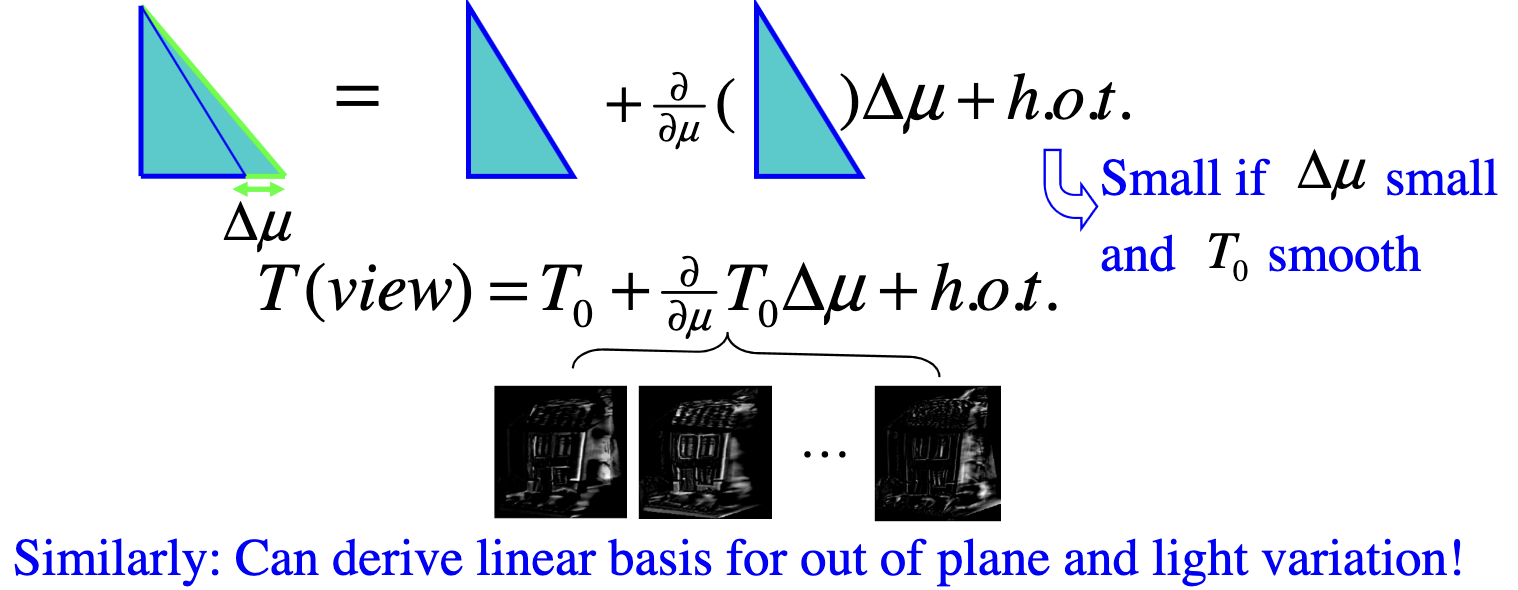
\includegraphics[width=.6\textwidth]{"imgs/taylor expansion mar12.png"}
  \end{center}
\end{list}

\subsection{Geometric spatial temporal variability}
Image 'warp'
\[
  T(\mathbf x) = I(W(\mathbf x ,\mu))
\]
Image variability caused by imperfect warp
\[
  \Delta T = I(W(\mathbf x, \mu + \Delta \mu)) - T_w
\]
First order approx.
\[
  \Delta T = I(W(\mathbf x, \mu)) + \nabla T \frac{\partial W}{\partial \mu} - T_w=
  \nabla T \frac{\partial W}{\partial \mu}
\]
Concrete examples: img plane; out of plane
\subsection{Variability due to a planar projective warp (homography)}
\subsection{Out of Plane Variability}
\subsection{Photometric Variation}
light changes how obj looks (?)
\\
dont need to raytrace


\subsection{Composite Variability}
composite texture intesity variability
\[
  \Delta \mathbf T = \Delta \mathbf T_s + \Delta \mathbf T_d + \Delta \mathbf T_l + \Delta \mathbf T_e
\]
planar + depth + light + res. err.
\\[5pt]
Can be modeled as sum of basis
\begin{flalign*}
  \Delta \mathbf T &= \mathbf{B_s y_s} + \mathbf{B_d y_d} + \mathbf{B_l y_l} + \Delta \mathbf(T_e)
  \\
  &= \mathbf{By + \Delta T_e}
\end{flalign*}

\subsection{How to Compute}
Slide 31 - 32 



\subsection{Dyntex}



\pagebreak
\section{Lecture - Mar 19}
lec07modeling18EmbMedia
% \\[10pt]

\subsection{Summary, 2 view rec}
$F$ independent of point correspondence, maps them to each other; same for all
\\
can use real measurements to rectify 

\subsection{Multiview Stereo}
Nonsequential image selections - features lost and reinitialized as new features
\begin{list}{}{}
  \item SOVE by matching with other \textit{close} views
\end{list}


\subsubsection{Relating more views}
Relating nearby images
\\
For every view $i$
\begin{list}{}{}
  \item extract features
  \item compute 2 view geom $i-1$ / $i$ and matches 
  \item Compute pose using robust algo
  \item For all close views $k$:
  \item \begin{list}{}{}
    \item compute two view geom $k$ / $i$ and matches
    \item infer new 2D - 3D matches and add to list 
  \end{list}
  \item Refine pose using all 2D - 3D matches
  \item Refine existing structure
  \item Initialize new struct
\end{list}
If viewpoints are close; most img changes can be modelled through a planar homography
(can approx. map close imgs via homography)
\\
Qualitative distance measure is obtained via residual error on best possible planar
homography 
\\
Find 'best' homography (?)

\noindent\rule{\textwidth}{0.2pt}

\subsection{Refining structure and Motion}
Minimize reprojection error
\[
  \min_{\hat P_k, \hat M_i}
\]
via MLE (if error zero mean gaussian noise); nonlinear opt.
\\
Huge problem but can be solved efficiently (bundle adjustment)
\\
Sometimes do this for simple scenes 
(usually use fundamental matrix method but can use several sets of affine models)
\\
Quality of final doesnt depend on initial


\subsection{Bundle Adjustment}
\textbf{Refining a captured model}
\\
Search method; change X and P until we get best match
\\
Refine structure $X_j$ and motion $P^i$ 
\\
Minimize geometric error
\\
ML solution, assuming noise is Gaussian
\\
Tolerant to missing data 
\[
  \min \sum_{i,j} d(PX, x)^2
\]


\subsection{Projective ambiguity and self-calibration}
\textbf{autocalibration} - determine projective transformation $T$ that
upgrades the projective reconstruction to a metric one


\subsection{Complete modeling system}
Seq. of frame $\to$ scene struct
\begin{enumerate}
  \item Get corresponding points (via. tracking or detect/match)
    \subitem tracking helpful for maintaining feature correspondence
  
  \item Affine factorization (alr. computes ML estimate over all frames; no need for
  bundle adjustment for simple scenes)

  \item Self calibration
  
  \item If several model segments: merge, bundle adjust

\end{enumerate}

\subsection{Stereo rec}
Sparse SFM $\to$ detailed map
\\
Get depth map via stereo


\subsection{Stereo image rect}
Reproject images planes onto a common plane; planes parallel w/ line b/w optical center 
\\
All epipolar lines are \textbf{parallel} in the rectified image plane.
\\
Rotate to make parallel $\to$ scan line matching
\\[5pt]
Take epipolar point $\to$ make infinite point $\to$ parallel epipolar lines
\\
Do this in a way that minimizes distortion

\section{Lecture - Mar 21}
lec07modeling18EmbMedia
\subsection{Stereo image rect cont.}
% When we use tracking 
Make use of epipolar geometry, move 2 separate image planes onto same plane to simplify
search problem $\to$ epipolar lines go from defined by Fund matrix to being in 
canonical (rows corr. to rows)
\\[5pt]
Find epipolar point thats finite, get homography that maps it to point at infinity
\\[5pt]
Could choose any plane to rep. ray sets, but want planes that are similar to the 
imgs (dont compress x,y axis too much)

\subsection{Stereo Matching Algos}
Match pixels in conjugate epipolar lines
\begin{list}{}{}
  \item assume brightness constancy
  \item many approaches
\end{list}

\subsubsection{Basic algo}
For each epipolar line:
\begin{list}{}{}
  \item For each pixel in the left img:
  \item \begin{list}{-}{}
    \item compare with every pixel on same epipolar line in right img
    \item pick pixel with minimum match cost
  \end{list}
\end{list}
Improvement: match windows
\\
Solve as energy minimization

\subsubsection{Stereo as energy min}
Find disparities $d$ that minimize an energy func. $E(d)$
\\
Simple pixel / window matching:
\[
  E(d) = \sum_{(x,y)\in I} C(x,y,d(x,y))
\]
$C(x,y,d(x,y))$ is the SSD distance b/w windows $I(x,y)$ and $J(x,y + d(x,y))$
\\
$C(x,y,d)$ - the disparity space image (DSI)
\[
  d(x,y) = \argmin_{d'} C(x,y,d')
\]
Simple pixel window matching - choose min of each col in DSI independently

\subsection{Stereo Matching}
Epipolar line gives 1D matching \\
Ordering
\\
Uniqueness
\\
Disparity Limit
\\
Disparity Gradient Limit
\\
Trade offs:
\begin{list}{}{}
  \item matching cost (data)
  \item discontinuities (prior)
\end{list}




\subsection{Disparity Map}
$(x',y') = (x+D(x,y),y)$

\subsection{Hierarchical stereo matching}
Down sample w/ gaussian pyramid
\\
Faster comp.
\\
Deals w/ large disparity ranges

\subsection{}
Sparse point cloud $\to$ can use splatting 

\subsection{SLAM - Online scene modeling}
Triangulate points and reproject texture

\section{Lecture - Mar 26}
\subsection{Methods of Modelling - MVS}
\subsubsection{Shape reconstruction}
Given:
\begin{list}{}{}
  \item set of imgs of an obj / scene
  \item camera calibration info
  \item light cal. info
\end{list}
Find surface that best agrees w/ input imgs
\\
Approach:
\begin{list}{}{}
  \item choose surface representation $\mathcal S, X$
  \item define photo consistency func (+ regularization in practice) $\phi (X)$
  \item solve minimization
  \[
    \min_\mathcal S \int_{X\in\mathcal S} \phi(X)dX
  \]
\end{list}

\subsubsection{Photo Consistency Function}
\[
  \phi (X)
\]
Based on img cues (shading, stereo, silhouette, $\ldots$)
\\
Extension SFS/PS to multi view: (need cam + light calibration)
\begin{list}{}{}
  \item move cam $\to$ SFS
  \item move obj. $\to$ PS
\end{list}

\subsubsection{Surface Repr}
Image-centered
\begin{list}{}{}
  \item depth/disparity wrt image plane
  \item partial obj rec - limited res, viewpoint dependent
\end{list}
Object-centered
\begin{list}{}{}
  \item Voxels
  \item Level sets (implicit - fold)
  \item Mesh
  \item Depth wrt a base mesh
  \item Local patches
\end{list}


\subsubsection{Volumetric Representation}
obj: collection of voxels\\
normals: ?\\
method: carve away voxels that arent photoconsistent w imgs (discrete)\\
regularization: no way of ensuring smoothness
\\
visibility: ensured by the order of traversal (in general a problem)

\subsubsection{Disparity/Depth map}
obj (surface): $s(x,y) = (x,y,f(x,y))$
\\
normals: \[
  \mathbf u = s_x \times s_y = [s_x, s_y, -1]^\top
\]
method: find $f$ tht best agrees w input imgs (min the cost functional integrated over surface)
\[
  \min \int_x\int_y \phi (x,y,f,\nabla f) dxdy
\]
regularization: smoothness on $\nabla f$
\[
  \phi_{smooth} = \nabla f^2
\]
visibility: ? (fine mesh)


\subsubsection{Depth wrt base mesh}
obj (surface): $X=X^B + fd$ d = displacement dir. (displacement map)
\\
normals: local (per triangle)
\[
  \mathbf n = [f_x, f_y, -1]^\top 
\]

transform to global cs
\\
methods: 
\[
  \min_f \int_{X^B} \phi (X^B, f, \nabla f)dxdy
\]
regularization: smoothness on $\nabla f$ (local / global)
\\
visibility: ? (fine mesh)


\subsubsection{Mesh}
obj: mesh vertices
\[
  X = \lambda_3 v_1 + \lambda_2 v_2 + \lambda _3 v_3
\]
normals: interpolated
\[
  n = \lambda_1 n_1 + \lambda _2 n_2 + \lambda_3 n_3
\]
\[
  n_j = \sum_{j,k,i\in\Delta (v_j)} (v_k - v_j) \times (v_i - v_j)
\]
methods:
\\
(finish)

\subsection{voxel coloring}
carve away voxels until photo consistent\\
depth ordering

\subsection{space carving: photo hull}
photo hull - union of all photo consistent shapes

\subsection{graph cut}
multiple possible regularizations

% \subsection{Photo consistency function}


\subsection{surface evolution}
















\end{document}
